\subsection{Вычислительные эксперименты}
    Возьмём такие функции для реализации модели:
    \[
        \begin{split}
            & \varepsilon (x_1) = -x_1 + 10, \\
            & K_{12} (x_1) = x_1 - 5, ~ K_{13} (x_1) = x_1 - 3, ~ K_{23} (x_2) = x_2 - 4, \\
            & V_{12} (x_1) = 2 x_1, ~ V_{13} (x_1) = 3 x_1, ~ V_{23} (x_2) = x_2.
        \end{split}
    \]

    Тогда точки равновесия и их собственные значения равны:
    \[
        \begin{split}
            & x^{(0)} = (0,0,0), ~ \lambda_i = (10, -5, -7), \\
            & x^{(1)} = (10,0,0), ~ \lambda_i = (5, 3, -10), \\
            & x^{(2)} = (7,0,1), ~ \lambda_i = (1, -3.5 \pm i \cdot 2.96\dots), \\
            & x^{(3)} = (5,2.5,0 ), ~ \lambda_i = (0.5, -2.5 \pm i \cdot 4.33\dots), \\
            & x^{(4)} = (5.5,1.5,0.5), ~ \lambda_i = (-0.348\dots, -2.57\dots ~ \pm i \cdot 4.13\dots), \\
        \end{split}
    \]

    \subsubsection{При вымершей первой популяции}

    \begin{figure}[H]
        \centering
        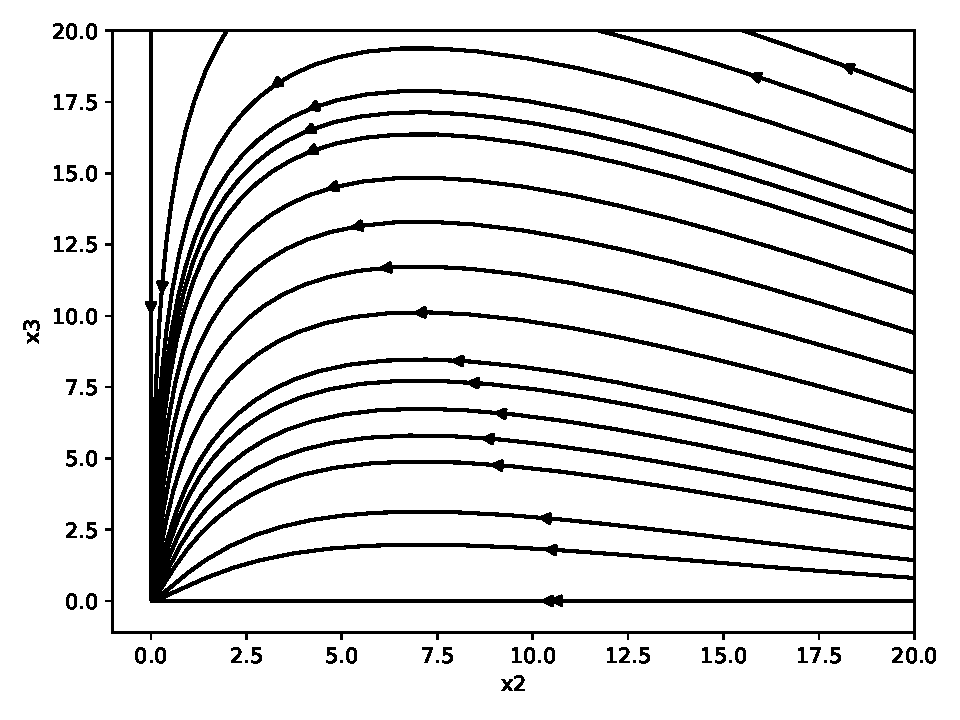
\includegraphics[width=8cm]{pictures/kx1_0vector.pdf}
        \caption{} \label{kx1_0}
    \end{figure}

    При \(x_1 = 0\) (Рис. \ref{kx1_0}) нулевая точка является устойчивым узлом. Обе популяции хищников в итоге вымрут.

    \subsubsection{При вымершей второй популяции}

    \begin{figure}[H]
        \centering
        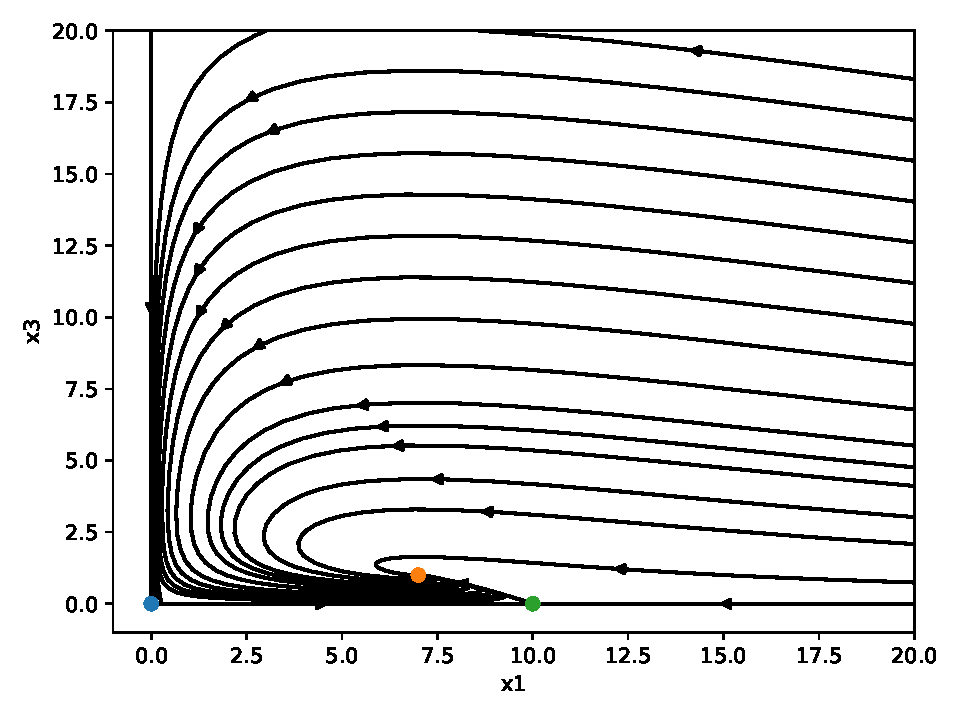
\includegraphics[width=8cm]{pictures/kx2_0vector.pdf}
        \caption{} \label{kx2_0}
    \end{figure}
    При \(x_2 = 0\) (Рис. \ref{kx2_0}) нулевая точка является седлом, точка \((10, 0)\) седлом, а \( \left( 7, 1 \right) \) -- устойчивым фокусом. Обе популяции со временем придут к точке баланса и их биомасса перестанет меняться.

    \subsubsection{При вымершей третьей популяции}

    \begin{figure}[H]
        \centering
        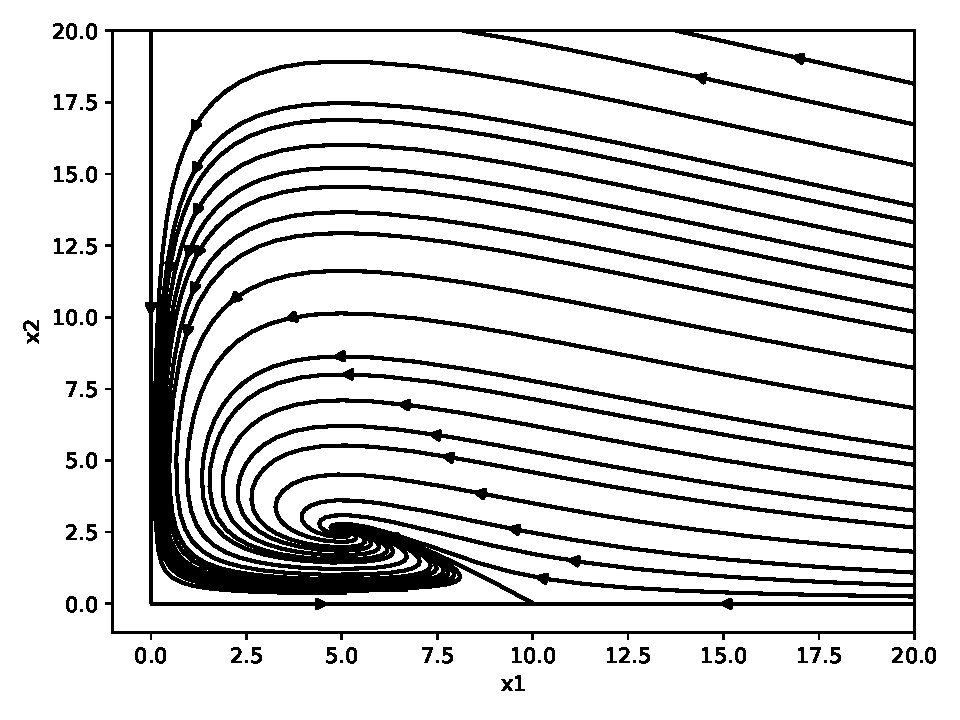
\includegraphics[width=8cm]{pictures/kx3_0vector.pdf}
        \caption{} \label{kx3_0}
    \end{figure}
    При \(x_3 = 0\) (Рис. \ref{kx3_0}) нулевая точка является седлом, точка \((10, 0)\) седлом, а \( \left( 5, 2.5 \right) \) -- устойчивым фокусом. Обе популяции со временем придут к точке баланса и их биомасса перестанет меняться.

    \subsubsection{Несколько изначально не вымерших популяций}
    Рассмотрим поведение решений во всей исследуемой области.
    \begin{figure}[H]
        \centering
        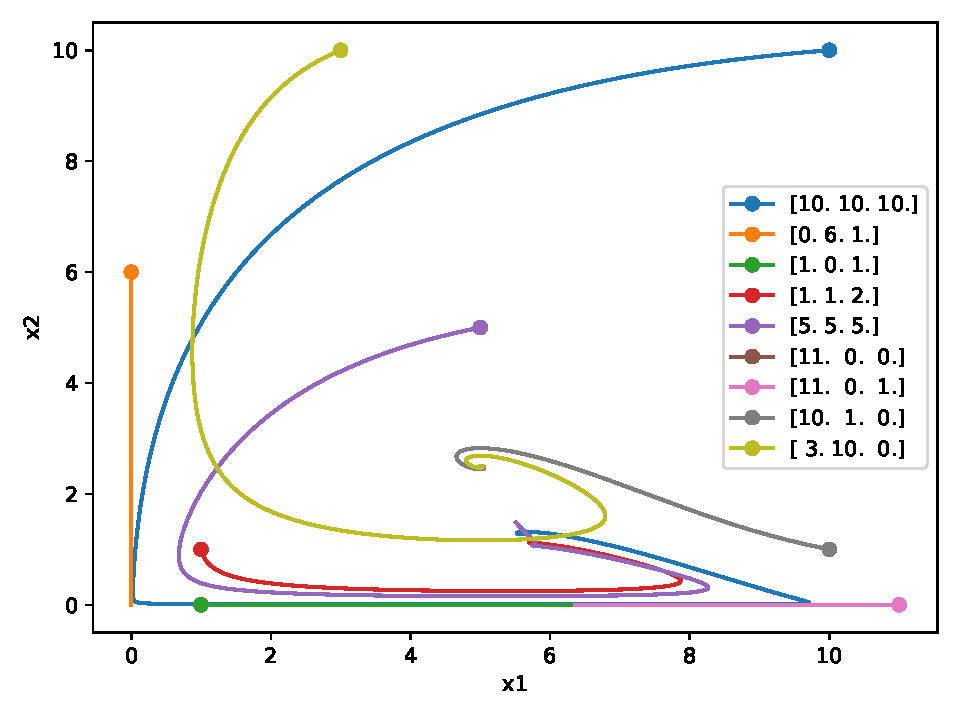
\includegraphics[width=8cm]{pictures/kx_12phase.pdf}
        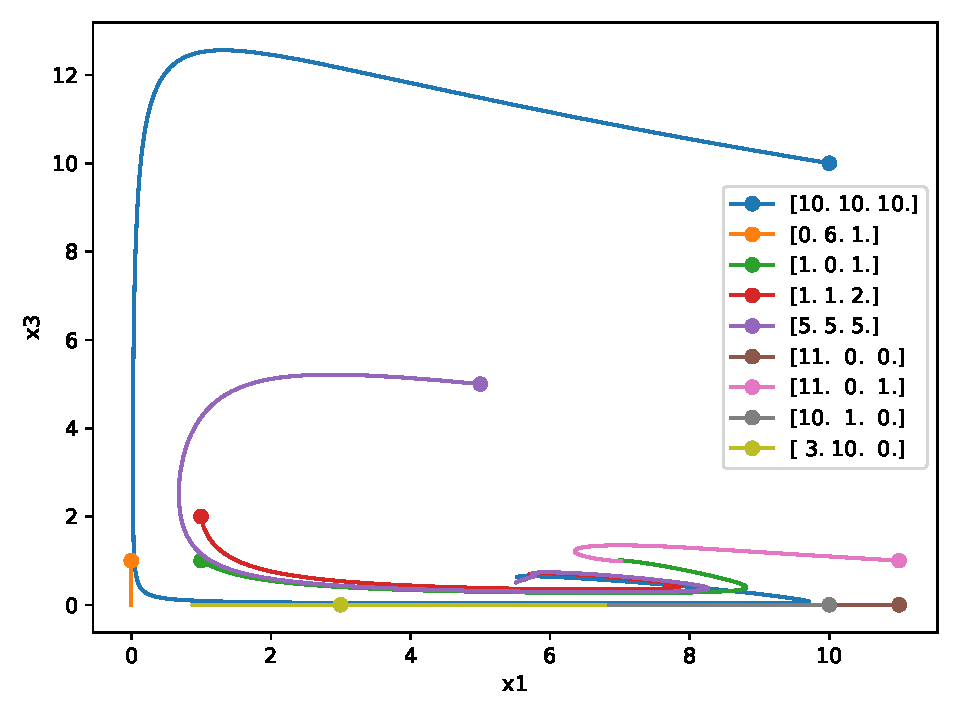
\includegraphics[width=8cm]{pictures/kx_13phase.pdf}
        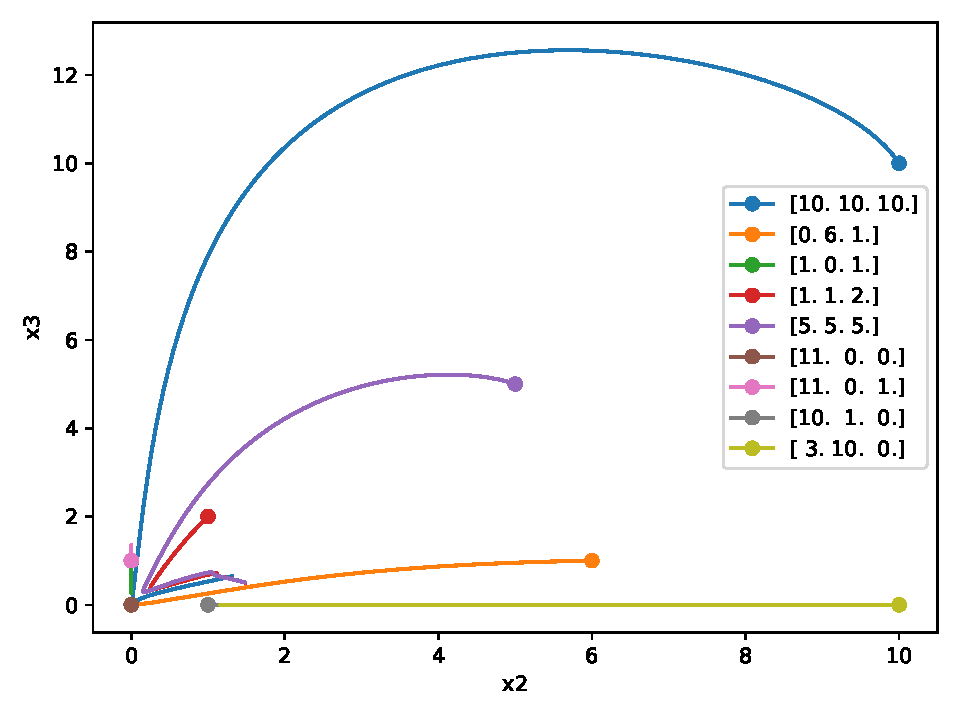
\includegraphics[width=8cm]{pictures/kx_23phase.pdf}
        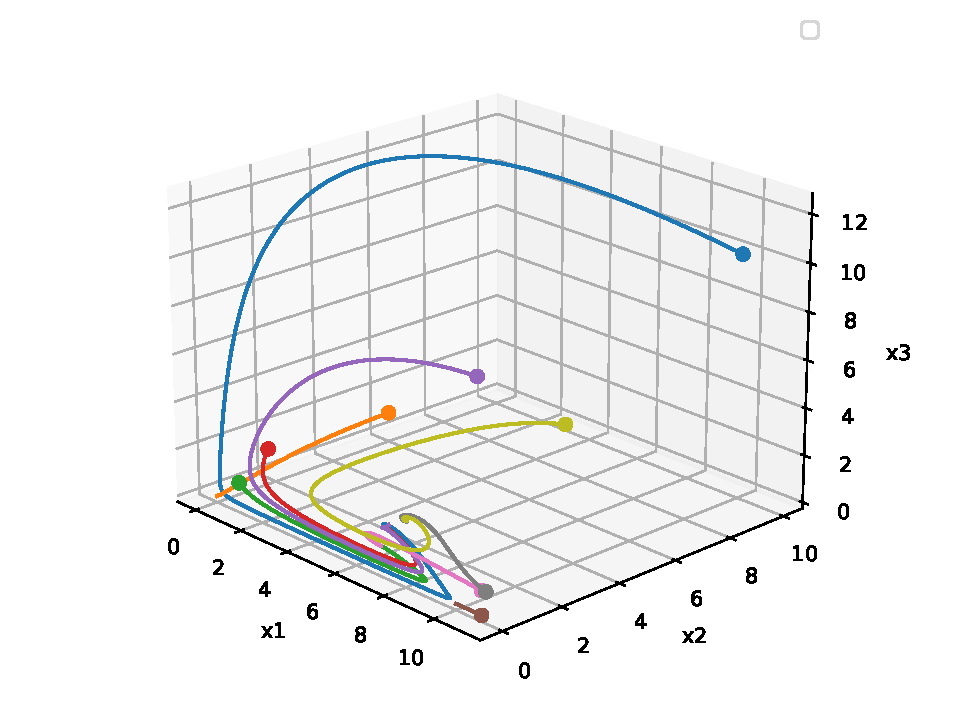
\includegraphics[width=8cm]{pictures/kx_phase3.pdf}
        \caption{На отрезке времени \( [0, 3] \).} \label{k3d1}
    \end{figure}

    На рисунке \ref{k3d1} изображены проекции на плоскости и 3-х мерная область с решениями. В отличие от исследованной модели Лотки-Вольтерры, начальные объёмы популяций, расположенные вне <<нулевых>> плоскостей, не способствуют вымиранию ни одной популяции. Рассмотрим как ведут себя решения вблизи ненулевой устойчивой точки равновесия.
    
    \begin{figure}[H]
        \centering
        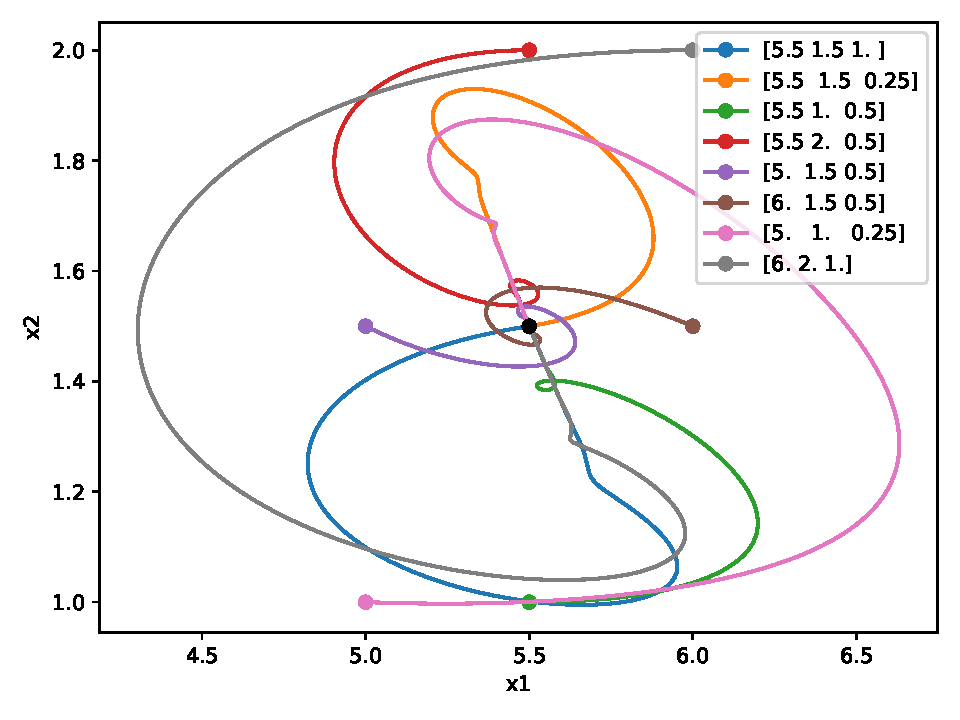
\includegraphics[width=8cm]{pictures/kx_12phase_g.pdf}
        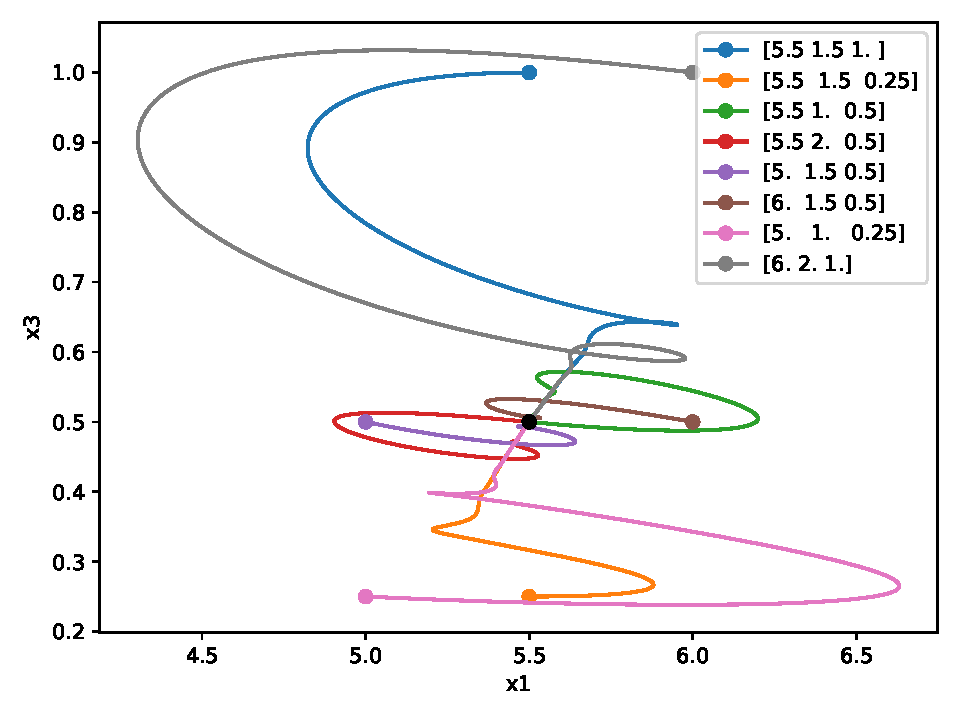
\includegraphics[width=8cm]{pictures/kx_13phase_g.pdf}
        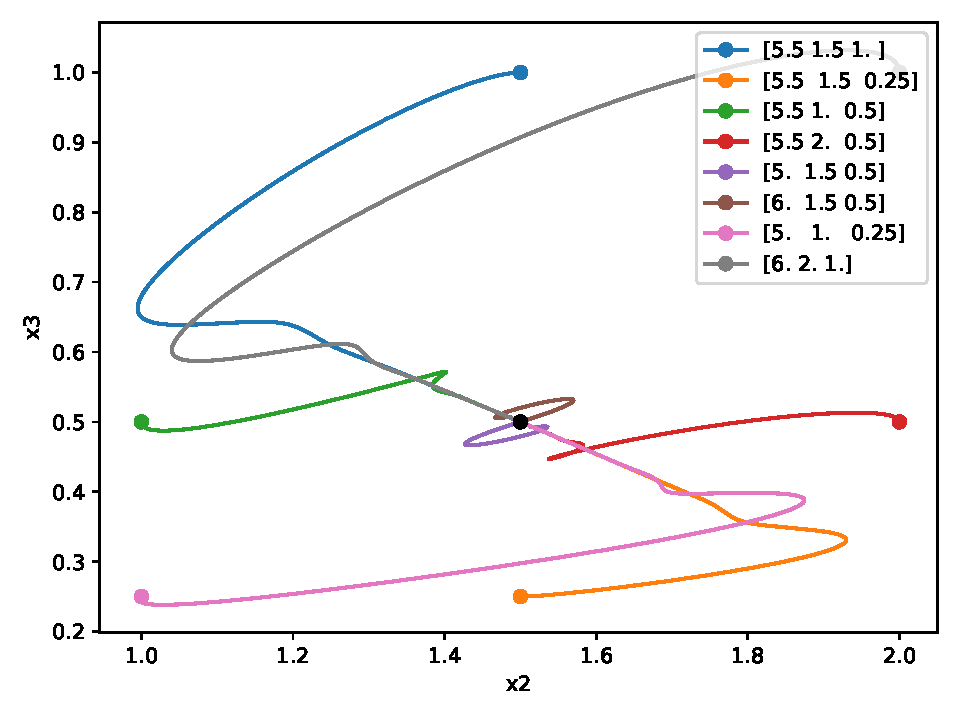
\includegraphics[width=8cm]{pictures/kx_23phase_g.pdf}
        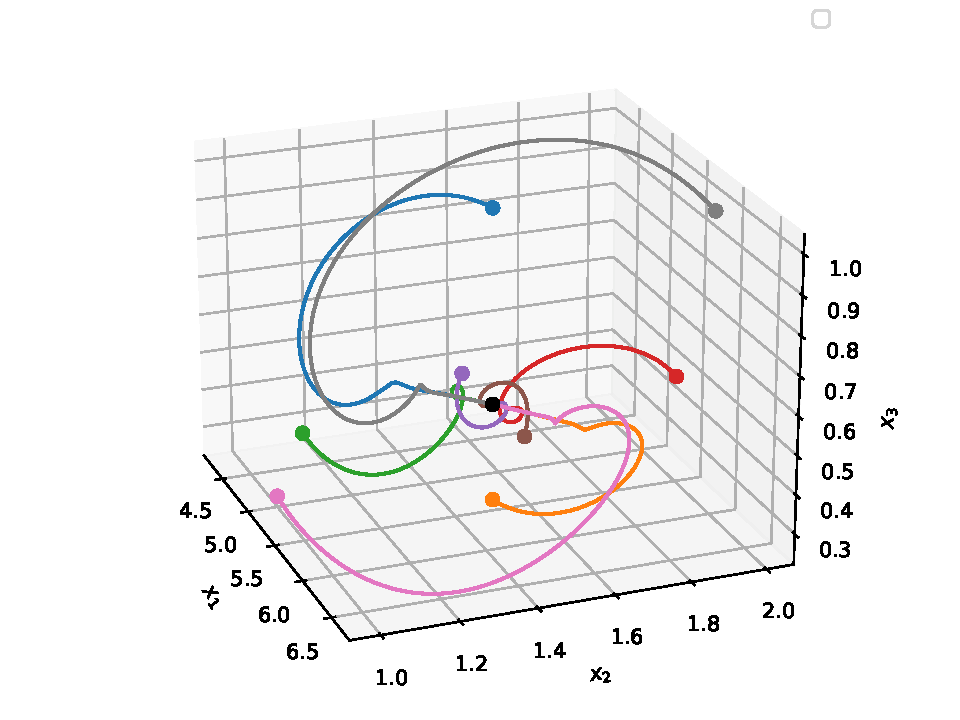
\includegraphics[width=8cm]{pictures/kx_phase3_g.pdf}
        \caption{Около точки \( (5.5, 1.5, 0.5) \). На отрезке времени \( [0, 3] \).} \label{k3d2}
    \end{figure}

    На рисунке \ref{k3d2} чёрной точкой изображена точка равновесия и несколько решений с указанными начальными значениями. Видно что все решения стремятся к ней, но также следуют по пути устойчивого фокуса, закручиваясь по спирали.  
    
    Теперь возьмём ненулевые начальные значения, но на большем удалении от этой точки равновесия.

    
    \begin{figure}[H]
        \centering
        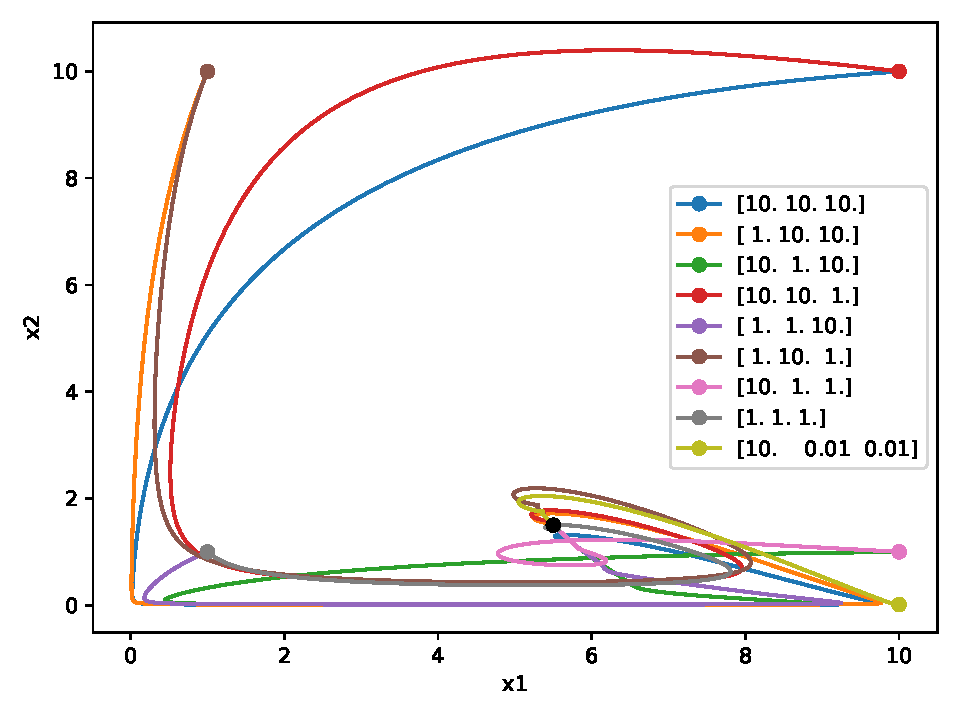
\includegraphics[width=8cm]{pictures/kx_12phase_g2.pdf}
        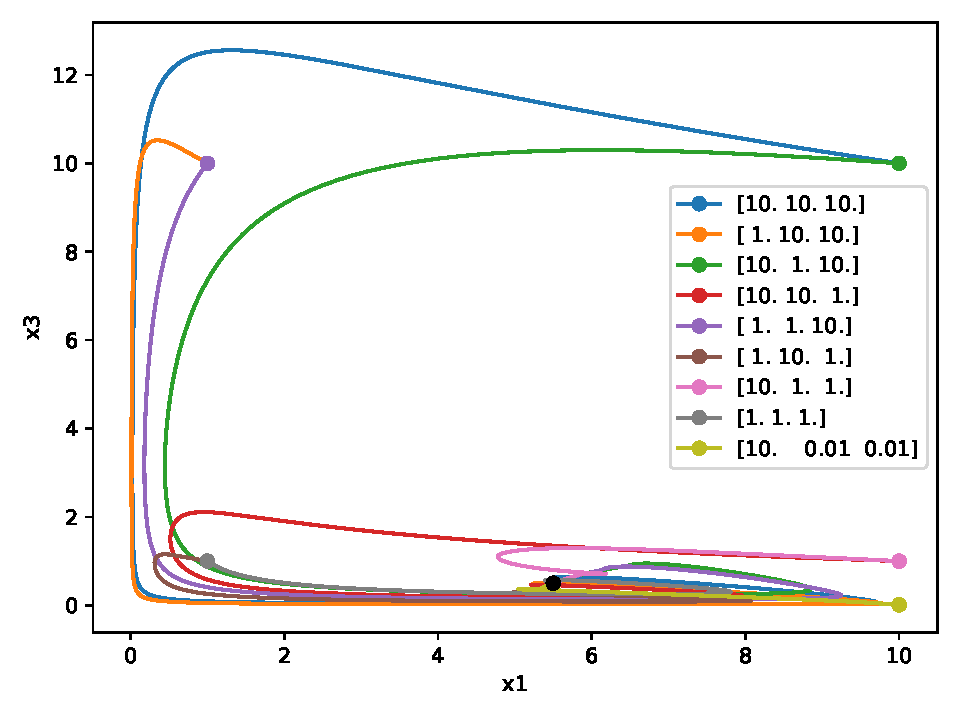
\includegraphics[width=8cm]{pictures/kx_13phase_g2.pdf}
        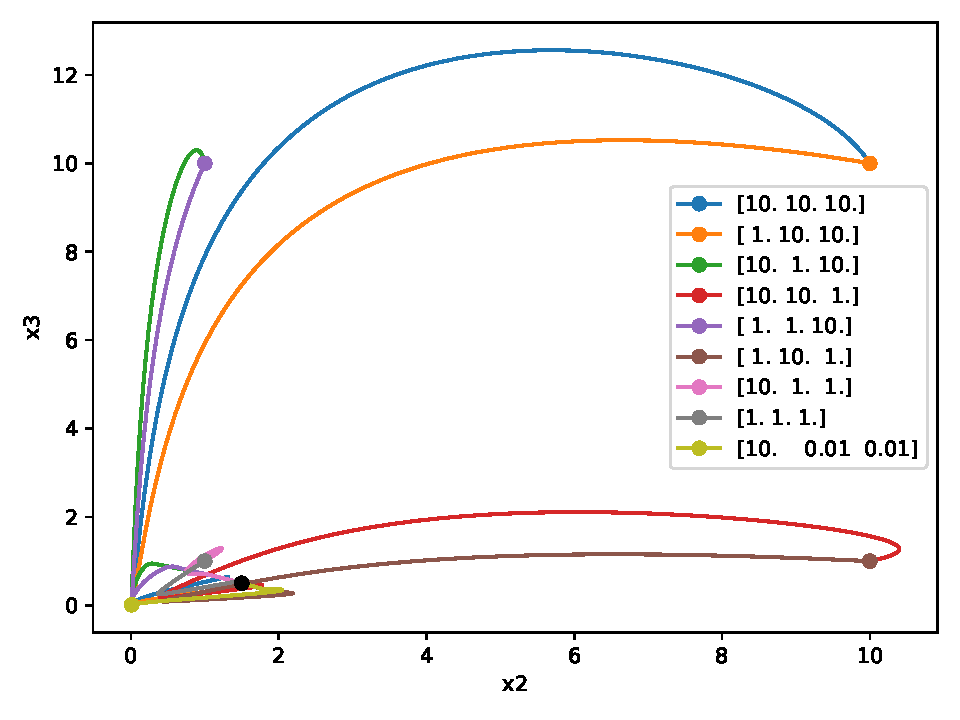
\includegraphics[width=8cm]{pictures/kx_23phase_g2.pdf}
        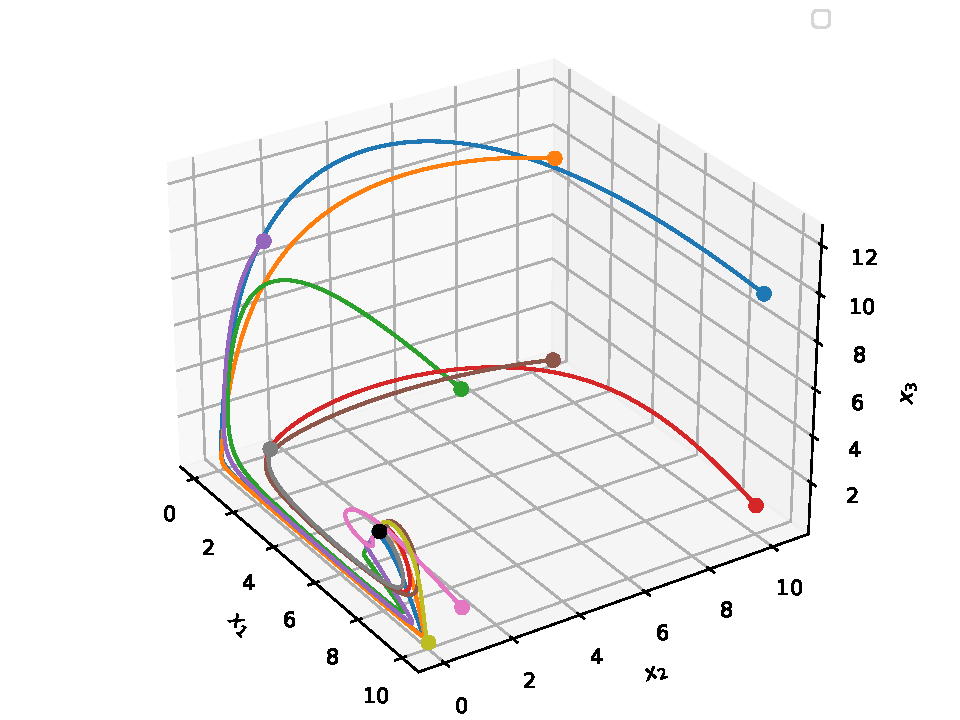
\includegraphics[width=8cm]{pictures/kx_phase3_g2.pdf}
        \caption{Несколько ненулевых начальных значений. На отрезке времени \( [0, 3] \).} \label{k3d3}
    \end{figure}

    На рисунке \ref{k3d3} все решения стремятся только к ненулевой точке равновесия. Значит, можно сделать вывод, что модель с данными параметрами при любых ненулевых начальных значениях приводит такие популяции к состоянию баланса, и их биомасса перестанет меняться. 
